\documentclass[11pt]{article}
\usepackage[margin=0.85in]{geometry}
\usepackage{amsmath,amssymb,booktabs,array,xcolor,tikz,hyperref,fancyhdr}
\usetikzlibrary{arrows.meta}
\definecolor{navy}{HTML}{17365D}
\hypersetup{colorlinks=true,linkcolor=navy,urlcolor=navy}
\pagestyle{fancy}\fancyhf{}\lhead{Multiple Linear Regression}\rhead{Study and Research Notes}\cfoot{\thepage}
\setlength{\headheight}{14pt}
\setlength{\parindent}{0pt}\setlength{\parskip}{6pt}
\newcommand{\R}{\mathbb R}\newcommand{\one}{\mathbf 1}\newcommand{\be}{\boldsymbol\beta}\newcommand{\eps}{\boldsymbol\varepsilon}
\begin{document}
\begin{center}
{\LARGE\bfseries Chapter 5: Multiple Linear Regression}\\[5pt]
{\large Foundations, Least Squares, Geometry, and the Overall $F$-Test}\\[5pt]
Study notes with extensions for later research\\
Version 1.0 $\mid$ October 14, 2026
\end{center}
\textbf{Scope.} These notes consolidate the concepts discussed so far, starting with the model and design matrix and ending at Section 5.6.1. The organization below is pedagogical; Sections 5.1--5.5 are not a verified transcription of the lecture's subsection headings. Section 5.6.1 follows the supplied screenshots. Research extensions are explicitly identified. Throughout, $p=m+1$ counts the intercept and $m$ predictor columns.
\tableofcontents
\newpage
\setcounter{section}{4}
\section{Multiple Linear Regression}
\subsection{The model, variables, and notation}
For observation $i$,
\[
Y_i=\beta_0+\sum_{j=1}^m\beta_jx_{ij}+\varepsilon_i,
\qquad i=1,\ldots,n.
\]
Here $Y_i$ is a response, $x_{ij}$ is predictor $j$ for observation $i$, $\beta_0$ is the intercept, and $\varepsilon_i$ is the unobserved error. A coefficient describes a change in the modeled mean while the other predictors are held fixed; this is not automatically a causal effect.

\textbf{Linear means linear in the unknown coefficients.} The model
\[
Y_i=\beta_0+\beta_1x_{i1}^2+\beta_2\log x_{i2}+\varepsilon_i
\]
is linear in its parameters (with $x_{i2}>0$). In contrast,
\[
Y_i=\beta_0+\beta_1e^{\beta_2x_{i1}}+\beta_3x_{i2}+\varepsilon_i
\]
is nonlinear in its parameters because the unknown $\beta_2$ is inside the exponential.

\textbf{Predictor versus covariate.} Both can be numerical or categorical. ``Covariate'' often emphasizes adjustment; traditional ANCOVA terminology reserves it for a numerical variable and calls a categorical variable a factor.

For a quantitative response, the following are conventional descriptions. Let $T_i$ indicate treatment and $S_i$ indicate smoking, each coded 0 or 1.
\begin{center}\small
\begin{tabular}{p{.20\linewidth}p{.23\linewidth}p{.47\linewidth}}
\toprule
Explanatory types&Common model name&Example mean $E(Y_i\mid X)$\\\midrule
Numerical + numerical&Multiple linear regression&$\beta_0+\beta_1\mathrm{Exercise}_i+\beta_2\mathrm{Age}_i$\\
Numerical + categorical&ANCOVA&$\beta_0+\beta_1\mathrm{Exercise}_i+\beta_2S_i$\\
Categorical + numerical&ANCOVA&$\beta_0+\beta_1T_i+\beta_2\mathrm{Age}_i$\\
Categorical + categorical&Additive two-way ANOVA&$\beta_0+\beta_1T_i+\beta_2S_i$\\\bottomrule
\end{tabular}\end{center}
All belong to the general linear model framework. Add $\beta_3T_iS_i$ if the treatment-group contrast is allowed to vary by smoking group. A factor with $k$ categories usually uses $k-1$ indicators when an intercept is included. The number $m$ counts design columns, not necessarily distinct scientific variables.

\subsection{The design matrix: rows, columns, and dimensions}
\[
Y=X\be+\eps,\qquad
X=\begin{pmatrix}1&x_{11}&\cdots&x_{1m}\\1&x_{21}&\cdots&x_{2m}\\\vdots&\vdots&&\vdots\\1&x_{n1}&\cdots&x_{nm}\end{pmatrix}.
\]
\begin{center}
\begin{tabular}{lll}\toprule
Object&Meaning&Dimension\\\midrule
$Y,\eps$&Response and error vectors&$n\times1$\\
$X$&Full design matrix&$n\times p$\\
$\be=(\beta_0,\ldots,\beta_m)^T$&Coefficient vector&$p\times1$\\
$\one_n$&Intercept column of ones&$n\times1$\\
$X_s$&Design excluding the intercept&$n\times m$\\\bottomrule
\end{tabular}
\end{center}
\textbf{Avoid a notation collision.} Lecture notes sometimes use $\mathbf x_i$ for an observation vector and $\mathbf x_j$ for a predictor column. They are different objects. Here we use
\[
r_i=\begin{pmatrix}1\\x_{i1}\\\vdots\\x_{im}\end{pmatrix}\in\R^p,
\qquad c_j=\begin{pmatrix}x_{1j}\\x_{2j}\\\vdots\\x_{nj}\end{pmatrix}\in\R^n.
\]
Then
\[
X=\begin{pmatrix}r_1^T\\\vdots\\r_n^T\end{pmatrix}
=(\one_n\;c_1\;\cdots\;c_m)=(\one_n\;X_s).
\]
The transpose makes an observation column vector into a row. It does not, by itself, indicate whether a vector represents an observation or a predictor.

\textbf{Example.} For ages 20, 30, 40 and weights 60, 70, 80,
\[
X=\begin{pmatrix}1&20&60\\1&30&70\\1&40&80\end{pmatrix},\quad
r_1^T=(1,20,60),\quad c_1=(20,30,40)^T,\quad c_2=(60,70,80)^T.
\]
The scalar $x_{12}=60$ is person 1's weight. Notice that this particular illustrative matrix is rank deficient: weight equals age plus 40, so it should not be used as a full-rank estimation example.

\subsection{Sample size, rank, and identifiability}
Full column rank means $\operatorname{rank}(X)=p$: no design column is an exact linear combination of the others.
\begin{center}\small
\begin{tabular}{p{.14\linewidth}p{.28\linewidth}p{.48\linewidth}}\toprule
Setting&Terminology&OLS consequence\\\midrule
$n\gg p$&Classical, low dimensional&Unique coefficients if full column rank holds.\\
$n>p$&Overdetermined&Full column rank is possible; residual df is $n-p$ if full rank.\\
$n=p$&Square; saturated if full rank&Full-rank fit interpolates $Y$; no residual df.\\
$n<p$&Underdetermined; often high dimensional&Rank is less than $p$; coefficients are not unique.\\\bottomrule
\end{tabular}\end{center}
Having $n>p$ does not guarantee rank $p$. For instance,
\[
X=\begin{pmatrix}1&1&2\\1&2&4\\1&3&6\\1&4&8\end{pmatrix}
\]
has $n=4>p=3$ but its last column is twice its second. Only $\beta_1+2\beta_2$ is identified, not the two slopes separately.

\textbf{Research extension.} Dimensionality is also about the ratio $p/n$ and how it changes with sample size. Problems with $p$ close to $n$ can show high-dimensional behavior even with $p<n$. This statistical issue is distinct from algebraic invertibility.

\subsection{Least squares: gradient, normal equations, and Hessian}
\subsubsection*{Step 1: minimize squared residuals}
\[
S(\be)=\|Y-X\be\|^2
=Y^TY-2\be^TX^TY+\be^TX^TX\be.
\]
The two cross terms combine because $Y^TX\be=\be^TX^TY$ is a scalar.
\subsubsection*{Step 2: differentiate}
For fixed $a$ and symmetric $A$,
\[
\nabla_{\be}(\be^Ta)=a,\qquad
\nabla_{\be}(\be^TA\be)=2A\be.
\]
Therefore,
\[
\nabla S(\be)=-2X^TY+2X^TX\be\in\R^{p\times1}.
\]
\subsubsection*{Step 3: solve the normal equations}
Setting the gradient to zero gives
\[
\boxed{X^TX\widehat\be=X^TY.}
\]
If $\operatorname{rank}(X)=p$,
\[
\boxed{\widehat\be=(X^TX)^{-1}X^TY.}
\]
Although $X$ is rectangular, $X^TX$ is $p\times p$ and square.
\subsubsection*{Step 4: verify the minimum using the Hessian}
\[
\boxed{\nabla^2 S=2X^TX.}
\]
For every $v\in\R^p$,
\[
v^T\nabla^2S\,v=2\|Xv\|^2\ge0.
\]
Thus $S$ is convex. If $X$ has full column rank, the expression is strictly positive for every $v\ne0$, so the Hessian is positive definite and the minimizer is unique.

If rank is deficient, there is a nonzero $v$ with $Xv=0$. Then
\[
X(\widehat\be+tv)=X\widehat\be\quad\text{for all }t\in\R.
\]
There are infinitely many minimizing coefficients, but a unique fitted vector. A useful global verification is
\[
S(\widehat\be+d)=S(\widehat\be)+\|Xd\|^2,
\]
because the normal equations make the cross term zero.

\subsubsection*{Worked example}
Let
\[
X=\begin{pmatrix}1&0\\1&1\\1&2\end{pmatrix},\quad
Y=\begin{pmatrix}1\\2\\2\end{pmatrix},\quad
X^TX=\begin{pmatrix}3&3\\3&5\end{pmatrix},\quad X^TY=\begin{pmatrix}5\\6\end{pmatrix}.
\]
The normal equations are
\[
3\widehat\beta_0+3\widehat\beta_1=5,\qquad
3\widehat\beta_0+5\widehat\beta_1=6.
\]
Subtracting gives $2\widehat\beta_1=1$, hence
\[
\widehat\beta_1=\tfrac12,\qquad \widehat\beta_0=\tfrac76.
\]
The Hessian is $\begin{pmatrix}6&6\\6&10\end{pmatrix}$ with leading principal minors $6>0$ and $24>0$, so the minimum is unique. The fitted values and residuals are
\[
\widehat Y=\begin{pmatrix}7/6\\5/3\\13/6\end{pmatrix},\qquad
e=\begin{pmatrix}-1/6\\1/3\\-1/6\end{pmatrix},\qquad SSE=\tfrac16.
\]
Check: $\one^Te=0$ and $(0,1,2)e=0$.

\subsection{Projection, orthogonality, centering, and inference foundations}
\subsubsection*{Geometry of the fit}
The column space $\mathcal C(X)=\{Xb:b\in\R^p\}$ contains every possible model prediction. OLS projects $Y$ onto this space:
\[
Y=\widehat Y+e,\qquad \widehat Y\in\mathcal C(X),\qquad X^Te=0.
\]
Residual orthogonality follows from optimization; the predictors themselves need not be mutually orthogonal.
\begin{center}
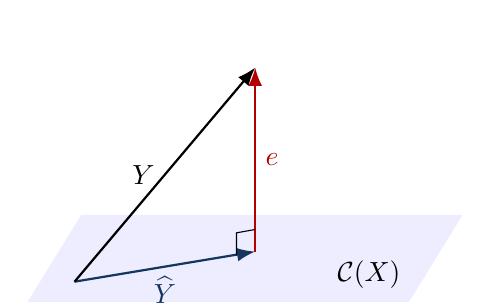
\begin{tikzpicture}[scale=.85,>=Latex]
\fill[blue!7] (-.7,-.3)--(5,-.3)--(5.8,1)--(.1,1)--cycle;
\node at (4.4,.1) {$\mathcal C(X)$};
\coordinate (O) at (0,0);\coordinate (P) at (2.7,.45);\coordinate (Y) at (2.7,3.2);
\draw[->,thick,navy] (O)--(P) node[midway,below] {$\widehat Y$};
\draw[->,thick] (O)--(Y) node[midway,left] {$Y$};
\draw[->,thick,red!70!black] (P)--(Y) node[midway,right] {$e$};
\draw (2.42,.40)--(2.42,.73)--(2.7,.78);
\end{tikzpicture}\\
\small Schematic: the residual is perpendicular to the entire fitted space.
\end{center}
When full rank holds, define the hat matrix
\[
H=X(X^TX)^{-1}X^T,\qquad \widehat Y=HY,\qquad e=(I-H)Y.
\]
Its essential properties are
\[
H^T=H,\quad H^2=H,\quad \operatorname{rank}(H)=\operatorname{tr}(H)=p,
\quad H(I-H)=0.
\]
A projection applied twice equals the same projection. The Hessian $2X^TX$ is $p\times p$; the hat matrix $H$ is $n\times n$. They are different matrices.

\subsubsection*{Centering and the intercept-only projection}
\[
H_1=\frac1n\one\one^T,\qquad H_1Y=\bar Y\one,\qquad C=I-H_1.
\]
Multiplication by $C$ subtracts the mean. In particular,
\[
X_c=CX_s=X_s-\one\bar x^T,\qquad
\bar x^T=(\bar x_1,\ldots,\bar x_m).
\]
Every column of $X_c$ sums to zero. This makes centered predictor columns orthogonal to the intercept column, but does not generally make them orthogonal to each other.
With full rank, the slopes and intercept can be recovered as
\[
\widehat\be_s=(X_c^TX_c)^{-1}X_c^TCY,\qquad
\widehat\beta_0=\bar Y-\bar x^T\widehat\be_s.
\]
\subsubsection*{Statistical assumptions}
Algebraic least squares does not require normality. For the following classical mean and variance results, condition on a fixed $X$ and assume
\[
E(\eps\mid X)=0,\qquad \operatorname{Var}(\eps\mid X)=\sigma^2I.
\]
Then
\[
E(\widehat\be\mid X)=\be,\qquad
\operatorname{Var}(\widehat\be\mid X)=\sigma^2(X^TX)^{-1}.
\]
If $n>p$,
\[
s^2=\frac{SSE}{n-p},\qquad E(s^2\mid X)=\sigma^2.
\]
\textbf{Crucial distinction:} $X^Te=0$ is a sample fitting identity; $E(\eps\mid X)=0$ is an assumption about the data-generating process. The former does not prove the latter.

\subsection{Testing the fit: the basic ANOVA table}
\subsubsection{The overall $F$-test}
\textbf{Question.} Do the predictors jointly improve on an intercept-only model?
\[
H_0:\beta_1=\cdots=\beta_m=0,
\qquad H_1:\text{at least one slope is nonzero}.
\]
The intercept is not tested. Under $H_0$, the modeled response mean is constant.

\paragraph{Sums of squares.}
For a full-rank OLS model with an intercept,
\begin{align*}
SST&=\sum_i(Y_i-\bar Y)^2=Y^T(I-H_1)Y,\\
SSR&=\sum_i(\widehat Y_i-\bar Y)^2=Y^T(H-H_1)Y,\\
SSE&=\sum_i(Y_i-\widehat Y_i)^2=Y^T(I-H)Y.
\end{align*}
The decomposition
\[
Y-\bar Y\one=(\widehat Y-\bar Y\one)+e
\]
is orthogonal, so the Pythagorean theorem gives
\[
\boxed{SST=SSR+SSE.}
\]
Thus $SSR=SST-SSE$ is the reduction in squared error relative to predicting the sample mean for everyone.

\paragraph{Mean squares and intuition.}
\[
MSR=\frac{SSR}{m},\qquad MSE=\frac{SSE}{n-m-1},\qquad
\boxed{F=\frac{MSR}{MSE}.}
\]
Under the stated mean and variance assumptions,
\[
E(MSE)=\sigma^2,\qquad
E(MSR)=\sigma^2+\frac{\be_s^TX_c^TX_c\be_s}{m}.
\]
The extra term is nonnegative because
\[
\be_s^TX_c^TX_c\be_s=\|X_c\be_s\|^2
=\sum_i\left[\sum_j\beta_j(x_{ij}-\bar x_j)\right]^2.
\]
It measures variation in the true modeled means around their average. Under $H_0$ both mean squares estimate $\sigma^2$. Under $H_1$, the regression mean square contains additional signal. Large $F$ is therefore evidence against $H_0$. This does not assert $E(F)=1$ under the null.

\paragraph{Why an $F$ distribution?}
For the exact finite-sample distribution assume $\eps\sim N_n(0,\sigma^2I)$. Under $H_0$,
\[
SSR/\sigma^2\sim\chi_m^2,\qquad SSE/\sigma^2\sim\chi_{n-p}^2.
\]
These quadratic forms are independent because the corresponding projections are orthogonal:
\[
(H-H_1)(I-H)=0.
\]
Consequently,
\[
\boxed{\frac{SSR/m}{SSE/(n-m-1)}\sim F_{m,n-m-1}\quad\text{under }H_0.}
\]
The unknown $\sigma^2$ cancels in the ratio.

\paragraph{Quadratic-form result behind the test.}
If $Z\sim N_n(\mu,\sigma^2I)$ and $P$ is symmetric and idempotent with rank $r$, then
\[
\frac{Z^TPZ}{\sigma^2}\sim\chi_r^2(\lambda),\qquad
\lambda=\frac{\mu^TP\mu}{\sigma^2}.
\]
Here the noncentrality parameter uses the standard convention without a factor $1/2$. If $\lambda=0$, the chi-square is central. For symmetric projection matrices $P,Q$, the condition $PQ=0$ gives independence of the corresponding normal quadratic forms. Normality is essential to this independence argument.

\paragraph{ANOVA and decision.}
\begin{center}
\begin{tabular}{lllll}\toprule
Source&df&Sum of squares&Mean square&Test statistic\\\midrule
Regression&$m$&$SSR$&$SSR/m$&$MSR/MSE$\\
Residual&$n-m-1$&$SSE$&$SSE/(n-m-1)$&\\
Total&$n-1$&$SST$&&\\\bottomrule
\end{tabular}
\end{center}
At level $\alpha$, reject for $F_{\mathrm{obs}}>F_{\alpha;m,n-m-1}$, where $F_\alpha$ denotes an upper-tail critical value. Equivalently, reject if the upper-tail $p$-value is less than $\alpha$.

\textbf{Example.} With $n=10$, $m=2$, $SSR=60$, and $SSE=14$,
\[
MSR=30,\qquad MSE=2,\qquad F=15,
\]
compared against $F_{2,7}$ under the null. Rejection supports at least one nonzero slope, not that every predictor is important or that the relationship is causal. Failure to reject is not proof that all slopes are zero.

\paragraph{Power under the alternative.}
Under a fixed nonzero slope vector,
\[
F\sim F_{m,n-p}(\lambda),\qquad
\lambda=\frac{\be_s^TX_c^TX_c\be_s}{\sigma^2}.
\]
Larger signal relative to error increases power. Under a stable, nondegenerate design with fixed $m$ and fixed nonzero slopes, $n^{-1}X_c^TX_c\to Q$ positive definite implies $\lambda$ grows proportionally to $n$ and power tends to one. A mere upper bound $X_c^TX_c=O(n)$ alone does not establish this conclusion.

\newpage
\section*{Research extensions: using the foundations responsibly}
\addcontentsline{toc}{section}{Research extensions}
\textbf{Purpose.} The following are conceptual extensions, not a complete analysis protocol or a substitute for design-specific methods.

\subsection*{Diagnose the actual problem}
\begin{center}\small
\begin{tabular}{p{.23\linewidth}p{.30\linewidth}p{.37\linewidth}}\toprule
Issue&Meaning&Response\\\midrule
Nonorthogonal columns&Usual correlations among predictors&OLS is valid algebraically if full rank.\\
Exact dependence&Coefficients are not separately identified&Remove redundant encoding or reparameterize; identify estimable combinations.\\
Near dependence&Some coefficient directions have little information&Assess uncertainty and sensitivity; consider ridge or better data.\\
$p>n$&Too many coefficient directions for unique OLS&Add explicit structure; evaluate prediction and uncertainty appropriately.\\
Misspecified mean&Chosen column space omits relevant structure&Use scientifically motivated transformations, interactions, or splines.\\
Unequal error variance&Classical covariance formula may fail&Consider appropriate robust covariance or justified weighted least squares.\\
Dependent observations&$\sigma^2I$ is inappropriate&Use methods reflecting clustering, repeated measures, time, or sampling design.\\\bottomrule
\end{tabular}
\end{center}

\subsection*{Numerical computation and near dependence}
The inverse formula is useful for theory. In computation, solve least squares using QR decomposition or SVD rather than explicitly inverting $X^TX$. If $X=QR$ has full column rank and $Q^TQ=I$, solve
\[
R\widehat\be=Q^TY,\qquad \widehat Y=QQ^TY.
\]
Orthogonal computational directions can be constructed even when the original predictors are correlated. SVD also reveals small singular values and rank deficiency. Forming $X^TX$ squares the 2-norm condition number in the full-rank case.

VIFs summarize inflation associated with linear relationships among slope columns: $VIF_j=1/(1-R_j^2)$, where $R_j^2$ comes from regressing predictor $j$ on the other predictors with an intercept. There is no universal VIF cutoff that determines which scientific variable should be removed. Centering helps interpret intercepts and some polynomial terms, but does not remove ordinary correlations between the original numerical predictors.

\subsection*{Pseudoinverse and regularization}
A Moore--Penrose pseudoinverse gives $\widehat\be=X^+Y$, the minimum Euclidean norm OLS solution. It selects one coefficient vector without making redundant parameters identifiable. In a rank-deficient model, $\widehat Y=XX^+Y$ remains the unique orthogonal projection.

Ridge minimizes
\[
\|Y-X\be\|^2+\lambda\be^TD\be,
\quad D=\operatorname{diag}(0,1,\ldots,1),\quad\lambda>0,
\]
leaving the intercept unpenalized. Its solution is
\[
\widehat\be_\lambda=(X^TX+\lambda D)^{-1}X^TY.
\]
With a usual nonempty intercept column and all slopes penalized, this matrix is positive definite. The first-order condition is
\[
X^Te_\lambda=\lambda D\widehat\be_\lambda,
\]
so residuals are generally not orthogonal to all predictors, although they still sum to zero when the intercept is unpenalized. The ridge smoother is generally not an idempotent orthogonal projection.

LASSO replaces the squared slope penalty by $\lambda\sum_{j=1}^m|\beta_j|$ and can select zero coefficients. Its coefficient solution need not be unique without additional conditions. Tune penalties using a validation strategy suited to the data; standardize predictors within training folds when appropriate, and avoid information leakage.

\subsection*{Separate prediction, interpretation, and causality}
\begin{itemize}
\item \textbf{Prediction:} prioritize performance on new data; use suitable cross-validation and assess calibration and errors relevant to the application.
\item \textbf{Interpretation:} specify the target coefficient or contrast, justify adjustment variables, and report uncertainty and sensitivity to modeling choices.
\item \textbf{Causality:} define the intervention and estimand; justify identification using the study design and causal assumptions. Neither the overall $F$-test nor $X^Te=0$ rules out confounding.
\end{itemize}
Do not automatically remove an important confounder to reduce VIF. Do not treat post-selection ordinary standard errors as automatically valid after a data-driven search. A complex survey requires methods reflecting weights, strata, and clusters; ordinary iid formulas are not automatically appropriate.

\subsection*{A compact memory guide}
\begin{center}
\begin{tabular}{p{.25\linewidth}p{.65\linewidth}}\toprule
Concept&Question answered\\\midrule
Column space&What response patterns can the model express?\\
Projection&Which allowed prediction is closest to the observed $Y$?\\
Residual orthogonality&Why can no coefficient adjustment further reduce squared error?\\
Full column rank&Are the coefficients representing that fit unique?\\
Positive-definite Hessian&Is the least-squares objective strictly convex?\\
Residual degrees of freedom&How many dimensions remain for estimating error variance?\\
Overall $F$-test&Is the joint improvement beyond an intercept-only model statistically convincing?\\\bottomrule
\end{tabular}
\end{center}
\textbf{Final distinction.} Unique estimation, stable estimation, correct specification, and causal identification are separate properties. A model may satisfy one and fail another.

\end{document}
